% Vorlage: https://www.pfsr.de/latex

% -- Anfang Präambel
\documentclass[german,  % Standardmäßig deutsche Eigenarten, englisch -> english
parskip=full,  % Absätze durch Leerzeile trennen
%bibliography=totoc,  % Literatur im Inhaltsverzeichnis (ist unüblich)
%draft,  % TODO: Entwurfsmodus -> entfernen für endgültige Version
]{scrartcl}

\usepackage[utf8]{inputenc}  % Kodierung der Datei
\usepackage[T1]{fontenc}  % Vollen Umfang der Schriftzeichen
\usepackage[ngerman]{babel}  % Sprache auf Deutsch (neue Rechtschreibung)

% Mathematik und Größen
\usepackage{amsmath}
\usepackage[locale=DE,  % deutsche Eigenarten, englisch -> US
separate-uncertainty,  % Unsicherheiten seperat angeben (mit ±)
]{siunitx}
\usepackage{physics}  % Erstellung von Gleichungen vereinfachen

\usepackage{graphicx}  % Bilder einbinden \includegraphics{Pfad/zur/Datei(ohne Dateiendung)}

% Gestaltung
\usepackage{booktabs}  % schönere Tabellen
\usepackage[toc]{multitoc}  % mehrspaltiges Inhaltsverzeichnis
\usepackage{csquotes}  % Anführungszeichen mit \enquote
\usepackage{caption}  % Anpassung der Bildunterschriften, Tabellenüberschriften
\usepackage{subcaption}  % Unterabbildungen, Untertabellen, …
\usepackage{enumitem}  % Listen anpassen
\setlist{itemsep=-10pt}  % Abstände zwischen Listenpunkten verringern

% Manipulation des Seitenstils
\usepackage[headtopline = .5pt]{scrlayer-scrpage}

% Bibliographie
\usepackage[backend=biber]{biblatex}
\addbibresource{bibliography.bib}

% SI-Einheiten darstellen
\usepackage{siunitx}

% Kopf-/Fußzeilen setzen
\pagestyle{scrheadings}  % Stil für die Seite setzen
\clearmainofpairofpagestyles  % Stil zurücksetzen, um ihn neu zu definieren
\automark{section}  % Abschnittsnamen als Seitenbeschriftung verwenden
\ofoot{\pagemark}  % Seitenzahl außen in Fußzeile
\ihead{\headmark}  % Seitenbeschriftung mittig in Kopfzeile

\usepackage[hidelinks]{hyperref}  % Links und weitere PDF-Features

% TODO: Titel und Autor, … festlegen
\newcommand*{\titel}{Auswertung von pp-Kollisionsereignissen}
\newcommand*{\autor}{Sebastian Thiede, Alexander Lettau}
\newcommand*{\abk}{PP}
\newcommand*{\betreuer}{Max Märker}
\newcommand*{\messung}{02.12.2021 \& 09.11.2021}
\newcommand*{\ort}{ASB/429}

\hypersetup{pdfauthor={\autor}, pdftitle={\titel}}  % PDF-Metadaten setzen

% automatischen Titel konfigurieren
\titlehead{Praktikum des IKTP \abk \hfill TU Dresden}
\subject{Versuchsprotokoll}
\title{\titel}
\author{\autor}
\date{\begin{tabular}{ll}
Protokoll: & \today\\
Messung: & \messung\\
Ort: & \ort\\
Betreuer: & \betreuer\end{tabular}}

% -- Ende Präambel

\begin{document}
\begin{titlepage}
\maketitle  % Titel setzen
\tableofcontents  % Inhaltsverzeichnis setzen
\end{titlepage}

% ----- DOKUMENT ANFANG -----

\section{Aufgabenstellung}
Die Beschleunigermas­senspektrometrie (AMS) ist ein wichtiges Werkzeug zur Trennung und Detektierung von Nukliden.
Eine der häufigsten Anwendungen ist die Altersbestimmung von Proben aus der Natur durch Messung der Konzentration verschiedener Nuklide, die auf der Erdoberfläche durch kosmische Strahlung entstehen.
Im Gegensatz zu anderen Verfahren der Massenspektrometrie erreicht man bei der AMS eine sehr gute Unterdrückung atomarer und molekularer Isobare.
Die Messzeiten sind relativ kurz und es lassen sich auch kleine Proben untersuchen.

In diesem Versuch wurde der Beschleuniger DREAMS (DREsden AMS) vorgestellt.
Die generelle Handhabung wurde anhand folgender praktischer Aufgaben kennengelernt:
\begin{itemize}
  \item Inbetriebnahme eine Sputter-Ionenquelle und Erzeugung negativer Ionen
  \item Strahlentransport eines Isotopenpaares durch den Beschleuniger
  \item Kalibrierung der Verstärkung der gasgefüllten Ionistationskammer
  \item Aufnahme von Messwerten in der gasgefüllten Ionisationskammer
\end{itemize}

Zur Auswertung sind folgende Aufgaben zu bearbeiten:
\begin{itemize}
  \item Berechnung der Teilchenenergien nach dem Beschleuniger
  \item Plotten des Stromes des Ionenstrahls im Faraday Cup
  \item Abschätzung des Energieverlustes des Ionenstrahls in einer dünnen Folie
  \item Abschätzung des Energieverlustes des Ionenstrahls in Isobutan (Gas in der Ionisationskammer)
  \item Plotten der gemessenen Spektren und Identifikation der Ionen
  \item Berechnung der Konzentration von Radionukliden in einer unbekannten Probe
\end{itemize}

\section{Theorie}

\subsection{organische Szintillatoren}

Szintillatoren sind  Materialien die bei bestrahlung mit energiereichen Photonen oder geladenen Teilchen angeregt werden und die Anregungsenergie in Form von Licht wieder abgeben. Organische Szintillatoren bestehen wie der Name schon vermuten lässt vorwiegend aus Kohlenstoff, Wasserstoff, Sauerstoff und Stickstoff wie es auch in z.B. menschlichem Gewebe der Fall ist. Es liegt daher nahe Detektoren auf Basis organischer Szintillatoren für die Dosismessung im Strahlenschutz zu verwenden. Organische Szintillatoren bestehen typischerweise aus zwei Komponenten: Einem primären Fluoreszenzstoff (z.B. auf Basis von Polyvinyltoluol) und einem \glqq Wellenlängenschieber \grqq{} (z.B. POPOP) da die vom primären Fluoreszenzstoff abgegebenen UV-Strahlen in den meisten durchsichtigen Materialien eine nur sehr geringe Reichweite besitzen.

\subsection{Wechselwirkung von Photonen mit Materie}

Obwohl Photonen in vieler Weise mit Materie wechselwirken können sind für diesen Versuch nur zwei Prozesse von wesentlicher Bedeutung: Die Compton-Streuung und der Photoeffekt. In den folgenden Abschnitten werden beide näher erläutert.

\subsubsection{Photoeffekt}

Der Photoeffekt beschreibt die Anregung von Elektronen durch Absorption eines Photons.
Für den HPGe-Detektor ist vor allem der innere photoelektrische Effekt von Bedeutung. Er beschreibt die Zunahme der Leitfähigkeit eines Halbleiters durch Bildung von nicht aneinander gebundenen Elektron-Loch-Paaren. Der HPGe-Detektor besteht aus einem hochreinen Germanium-Kristall der zwischen einem $n^{+}$ Kontakt (typ. durch Lithium-eindiffusion) am positiven Spannungspol und einem $p^{+}$ Kontakt (typ. durch Bor-implantation) am negativen Spannungspol sitzt; Der Detektor insgesamt entspricht einer Halbleiterdiode in Sperrichtung. Trifft ein Photon auf den Detektor und erzeugt ein Elektron-Loch-Paar werden durch die anliegende Spannung Elektron und Loch abgesaugt und bilden so einen detektierbaren Verschiebungsstrom. Dafür muss das einfallende Photon natürlich genügend Energie besitzen um die Bandlücke zu überwinden (Für Germanium \SI{0.67}{\electronvolt}), praktisch jedoch deutlich mehr um das Siganl-Rausch-Verhältnis groß genug zu bekommen. So werden bei einfallenden Photonen von \SI{1}{\mega\electronvolt} etwa \num{3e5} Elektron-Loch-Paare erzeugt \cite{HPGe-Detektor}. Da bei Raumtemperatur eine ständige thermische Anregung der Elektronen enormes Signalrauschen verursachen würde ist eine Abkühlung mit flüssigem Stickstoff notwendig.
Für den zu kalibrierenden Detektor ist vor allem der äußere photoelektrische Effekt von Bedeutung, genauer für den Photoelektronenvervielfacher (Abb. \ref{theorie_PEV}).

\begin{figure}[ht]
	\centering
  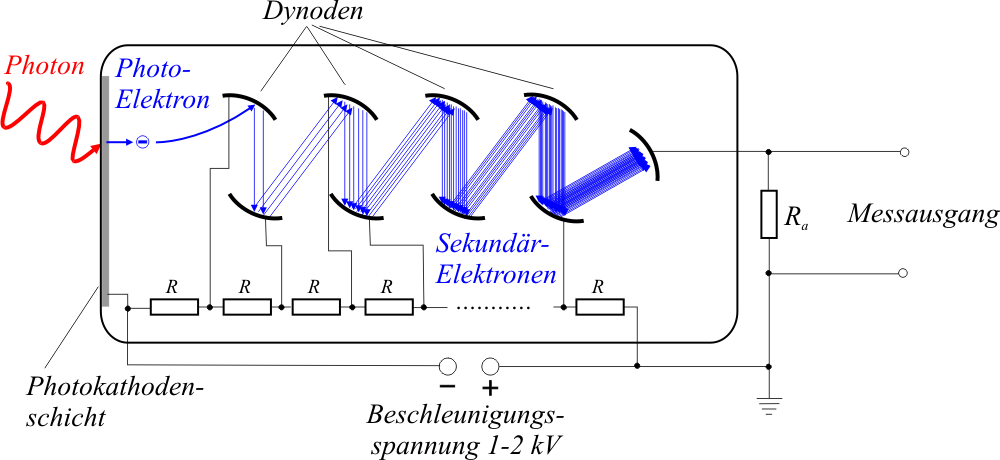
\includegraphics[width=0.85\textwidth]{images/Photomultiplier_schema_de.png}
	\caption{Schematik Photoelektronenvervielfacher}
	\label{theorie_PEV}
\end{figure}

Dort werden durch das Szintillationsphoton Elektronen aus einer Photokathode ausgeschlagen, durch angelegte Spannung zur ersten Dynode beschleunigt wo sie mit der gewonnenen kinetischen Energie weitere Elektronen auschlagen. Dieser Prozess wird einige male wiederholt bis ein messbarer elektrischer Impuls an der Anode entstehen kann.

\subsubsection{Compton-Streuung}

\subsection{Weitwinkel-Compton-Koinzidenz-Methode}

\section{Invariante Masse des $Z$-Boson}

In diesem Versuchsteil soll die invariante Masse von $Z^0 \rightarrow e^+ e^-$ Ereignissen berechnet werden.
Dies soll einmal exakt und einmal mit der Näherung $m_e = 0$ durchgeführt werden.
Für die Berechnung standen mehrere aufgenommene Detektorereignisse zur Verfügung, von denen zur Berechnung vier zufällig ausgewählt wurden.
Die invariante Masse beim Zerfall eines Teilchens in zwei Teilchen, ergibt sich mithilfe ihrer Vierervektoren zu:
\[
M^2 =\left[ \left( \begin{array}{c} E_1 \\ {\vec{p}_1} \end{array} \right) + \left( \begin{array}{c} E_2 \\ {\vec{p}_2} \end{array} \right) \right]^2
\]
\[
= m_1^2 + m_2^2 + 2 E_1 E_2 - 2 \textbf{p}_1 \textbf{p}_2 \cos \vartheta
\]
Die Energie ergibt sich aus der relativistischen Energie-Impuls-Relation zu:
\[
E_i = \sqrt{m_i^2 + \textbf{p}_i^2}
\]
Im Falle masseloser Teilchen, bzw. bei Vernachlässigung der Masse, vereinfacht sich die invariante Masse zu:
\[
M = \sqrt{2 \textbf{p}_1 \textbf{p}_2 (1-\cos \vartheta)}
\]

Hier sind $ \textbf{p}_i$ die Beträge der Impulse der Teilchen und $\vartheta$ ist der Winkel zwischen den Impulsvektoren.

Die Masse von Elektronen und Positronen beträgt: $m=511$ keV.
Zusammen mit den gegebenen Daten ergaben sich folgende invariante Massen:
\begin{center}
\begin{tabular}{ c | c| c | c | c | c }
Ereignis & $ \textbf{p}_1$ [GeV] & $ \textbf{p}_2$ [GeV] & $ \cos \vartheta $ & $M_{exakt}$ [GeV] &$ M_{m_e = 0}$ [GeV] \\ 
\hline
13 & 68,981 & 16,531 & -0,616 & 60,70137 & 60,70139 \\ 
16 & 49,689 & 60,917 & -0,140 & 83,06829 & 83,06830 \\
19 & 78,577 & 101,006 & 0,669 &72,48034 & 72,48037 \\
21 & 52,582 & 65,152 & 0,573 & 54,06895 & 54,06897 \\
\end{tabular}
\end{center}
Die Angabe der Nachkommastellen der invarianten Masse zeigt hier nicht die Messgenauigkeit, sondern soll die Unterschiede in der Berechnung zeigen.
Als Mittelwert ergibt sich eine Masse von $(67 \pm 11)$ Gev.

Wie zu sehen ist, bewirkt die Vernachlässigung der Masse in diesem Fall erst einen Unterschied in der sechsten Nachkommastelle, was für die Praxis kaum relevant ist und unter Umständen völlig von anderen Messunsicherheiten überdeckt wird.
Das ist auch nicht verwunderlich, da die Masse des Z-Bosons und damit auch die Energie die beim Zerfall zur Verfügung steht bei $91$ GeV liegt, während die Masse des Elektrons bei $511$ keV liegt.

Jetzt könnte als Frage aufkommen, warum die invarianten Massen doch recht weit von der Masse des Z-Bosons entfernt liegen.
Das Z-Boson äußert sich in der Messung als Resonanz mit endlicher Breite.
Aufgrund dieser Breite kann die Masse auch nicht exakt bestimmt werden, die gemessenen Werte werden um den wahren Wert gestreut.
Der Mittelwert von $M$ bei einer genügend großen Anzahl Messungen sollte dann jedoch der Z-Masse entsprechen.
\clearpage


\nocite{*} % alle resourcen auflisten
\printbibliography

% ----- DOKUMENT ENDE -----

\end{document}
